\section{More on matrices, graphs and stochastics}
\subsection*{Prologue}

Here we are starting transition from matrix terminology into that
of graphs and random walk. 
As in the previous section, there is an included appendix for this
chapter.
We show how to derive the properties of
RWR from the stochastic matrix theory and provide some examples for
propagation in graphs and setting the scene for the next section
where we deal with clustering. One reason why we provided the
relative expanded mathematical details on the previous section and
in this one is to explain why the restart is essential to turning a 
connected graph where a random walk generally doesn't reach a
steady state, into an acyclic graph (corresponding to a primitive
adjacency matrix). 


\subsection*{Theory}

A directed non-weighted graph $G$ can be uniquely represented by its
\textbf{adjacency matrix},
$A_{i,j} := 1$ if and only if there is a directed edge from $j$ to $i$ (if we
want to use it for transitioning on columns as done above). It's possible to
assign different edge weights rather than only $1$ and $0$. If the graph is
undirected each edge would be counted in both directions and the matrix is
symmetric.
Relabeling the vertices of a graph yields an adjacency matrix that is similar by
permutations ($PAP^{-1}$, where $P$ is a permutation matrix) and vice versa.

To turn $A$ into a transition, normalize each column by dividing it with
its out going rank, so let $D_{i,i} = \text{out~rank}(i)$, $T:=AD^{-1}$ is the
transition matrix of this graph (because right-multiplying by $D$ normalizes each
column by its rank).
If the graph was stochastic to begin with then the adjacency matrix as we
defined it is already column-normalized.

\begin{mydef}
\label{def:stronglyconnected}
A graph is $G$ \textbf{strongly connected} if there is a directed path form any edge
to any edge. Equivalently $G$ is strongly connected if and only if its adjacency matrix is irreducible.

We say that the \textbf{Period of a vertex} $v \in V(G)$ is the greatest common
divisor of all closed paths on $v$. If the periods of all vertices are equal
(spoiler: in the case that $G$ is strongly connected they are), we call it the
\textbf{Period of the graph} $G$.
\end{mydef}

\begin{remark}
\label{remark:periods}
If $G$ is strongly connected then the periods of all vertices are indeed equal
and its easy to prove. The corresponding adjacency matrix $A$ is irreducible so
it too has a period $h$ as defined in \ref{Ax:remark:wielandt_cyclicity} and it is
equal to the graph period (can be shown using \ref{Ax:thm:wielandt2} and
\ref{Ax:remark:wielandt_cyclicity}).

So if the graph $G$ is strongly connected and has period $1$
then the adjacency matrix is \textbf{aperiodic} and hence primitive, and vice versa. 
\end{remark}

From all the above we have seen that a Markov process can be represented in two
equivalent ways \textemdash as a transition matrix  and as the 
corresponding weighted directed graph.

If the graph $G$ is strongly connected and aperiodic, its corresponding
adjacency matrix is primitive. We know from \ref{thm:perron1} that there is a
unique stationary distribution $p$ and that the Markov process converges to $p$ no
matter from which distribution it starts. We may calculate $p$ using the
\textbf{power
method} which is efficient because it can be done in a matrix-free method. 
%We don't need to know the matrix itself just the dot product of it with a state
%vector.

If the graph $G$ is strongly connected, then \ref{thm:perron2} assures us the
existence and uniqueness of a stationary distribution $p$. But if $G$ is not
aperiodic, the corresponding adjacency matrix is not primitive. We cannot use
the efficient power method to calculate $p$. Also the process itself doesn't
stabilize on $p$. It is periodic and cycles between the $h$ eigenvectors on
the unit circle (see theorem \ref{Ax:thm:wielandt2}). 

We are therefore interested to find how to convert an \text{imprimitive}
matrix (= irreducible but not primitive)
to a primitive matrix or equivalently to turn a strongly connected but periodic graph
into an aperiodic graph.

Let $G$ be any weighted graph and $A$ its adjacency transition matrix. Some vertices may
be unreachable from other vertices and there might not exist a single and
unique stationary distribution.
A random walk on this graph is generally
dependent on the initial starting distribution $p_0$ and has the
form $p_{k+1} = Ap_k = \dots = A^k p_0$, where $p_k$ is the
distribution after $k$ steps.
If we allow the possibility of 'random restart' from any state, this
graph becomes totally connected it is guarantied to have a unique stationary
distribution to which any random walk converges regardless of the initial state.

When we talk about \textbf{random walk with restart (RWR)} we set a restart
state $q$ and a restart parameter $\alpha \in [0,1]$. At each step, we
either restart over to the state $q$, with probability of
$alpha$, or continue to walk using the normalized adjacency matrix
$A$. The state sequence is therefore
\begin{equation}
\label{eq:RWR}
p_{k+1} = \alpha q + (1 -
\alpha) A \cdot p_k
\end{equation}

It turns out that this random walk with restart is actually a normal
random walk but with an modified adjacency matrix (and respectively, an
modified weighted directional graph). 

\begin{lemma}
\label{lemma:Qq}
Let $q$ be any state, let $\alpha \in [0,1]$ and let  
$ Q = (q|q|\dots|q)$ (The square matrix whose every column equals $q$).
Then $Q$ is a transition and for any state $p$ we have $Qp = Q$.

In addition if $T$ is any transition then $W = \alpha Q + (1-\alpha)
T$ is also a transition, And we can rewrite the RWR from
\ref{eq:RWR} as

$p_{k+1} = \alpha q + (1 - \alpha) Ap_k = 
[\alpha Q + (1 - \alpha) A] p_k = W p_k$

\begin{proof}
Trivial and uses \ref{Ax:lemma:SplusT}
\end{proof}
\end{lemma}

The matrix $W$ represents a graph $G'$ where each edge of the
original graph $G$ is rescaled by a factor $1 - \alpha$ (and if $G$ is
undirected we treat each undirected edge as $2$ directed edges in
$G'$. In addition from each vertex $v$ we add edges to every other
vertex and the weight of the additional edge is $\alpha q[u]$.

If we pick the restart state $q$ in a way that makes $W$ primitive,
then \ref{thm:perron1} assures us that the RWR will converge,
$\lim_{k \to \infty} p_k =\lim_{k \to \infty} W^k p_0 = p$, where
$p$ is the unique stationary distribution of $W$. This means in
particular that we can use the power method to find out the
distribution $p$ by sequentially calculating $p_1, p_2, \dots$ until
it sufficiently converges, and it will converge to $p$ from any
initial state $p_0$ which we choose. 

Also we can take the limit $p = \lim_{k \to \infty}p_k$ and rewrite
\ref{eq:RWR} as:
\begin{equation}
\label{eq:RWR2}
\begin{aligned}
p = Wp = \alpha q + (1 - \alpha) A \\
[I - (1 - \alpha)A] p = \alpha q
\end{aligned}
\end{equation}

We will see later that we can invert the matrix in the second
equation of \ref{eq:RWR2} and use a direct solution for $p$ instead of
the power method. The power method has the advantage that we can use
the matrix $A$ implictly, because we only need to know $A \cdot p_k$
to compute $p_{k+1}$. $A$ is usually a sparse matrix because each
vertex usually only has few neighbors and so we can use matrix free
methods efficiently to calculate $p$ but that is beyong the scope of
this thesis.

In the particular case of pageRank, we choose a uniform restart
state $q = \mathbf{\frac{1}{n}}$. The corresponding matrix $Q =
(q|\dots|q) \gt 0$ is strictly positive, and therefore 
$W = \alpha Q + (1 - \alpha)A > 0$ is positive and therefore
primitive.

The stationary distribution which corresponds to this uniform
restart state $q$ is called the \textbf{PageRnak} for $G$ with
restart parameter $\alpha$. It is used to order the vertices
according to their 'relevance' in the network.



The PageRank is the stationary distribution of the process when we use unbiased
restart\textemdash A restart is equally likely from any vertex.
But we want more. We want to find out what happens when we restart, for example,
always from one single vertex $u$. We think of the stationary distribution $p_u$ that 
results from such process as the heat (or flow) which propagates out of $u$.
If we take another vertex $v$ we think of $p_u[v]$ as a measure of how close $v$
is to $u$, or how much heat $u$ sends to $v$.
Note that this is not symmetric $p_v[u] \neq p_u[v]$ in general.

%(memo: add an illustration about asymmetry)

\begin{lemma}
\label{lem:AplusP}
Let $A \geq 0$ be irreducible. Let $B \geq 0$ have a positive row (or column),
then $A + B$ is primitive.
\begin{proof}
In the appendix
\end{proof}
\end{lemma}

\begin{remark}
\label{rem:AplusP}
Lemma \ref{lem:AplusP} proves that we can propagate (namely do RWR) from any arbitrary restart
state $q$, including a single vertex and the combined transition matrix will be
primitive if the adjacency matrix $A$ is irreducible, or
equivalently, the corresponding graph $G$ is strongly connected.


Assume that $A$ is a normalized adjacency transition of a strongly
connected graph $G$.
Let $q$ be any state column vector, for example $e_1$ if we restart
from a single vertex, and let $Q = (q | q | \dots | q)$.
So $Q$ has a positive row and therefore $(1-\alpha)A + \alpha Q$ is a primitive
transition according to \ref{lem:AplusP}.

%Also worth noting that if $x \geq 0$ is any transition, then $Qx = q$.
\end{remark}

\begin{mydef}
\label{def:Transitionbiased}
Let $G$ be a graph with adjacency matrix $A$, and let $D$ be the
diagonal matrix of the out ranks of the vertices of $G$. Then we can
column normalize $A$ and create the transition $T = AD^{-1}$.
We define \textbf{the transition matrix with restart parameter}
$\alpha$ \textbf{and bias} $q$ as
\[
T_{\alpha, q} :=
(1 - \alpha)T + \alpha Q
\]
\end{mydef}

In general, 
the matrix $T_{\alpha,q}$ may have more than one unique stationary distribution $p$ 
(there is one for each strongly connected
component of its corresponding graph). But if we require that $G$ be
strongly connected (which means $A$ is irreducible),
then $T_{\alpha,q}$ is primitive by \ref{lem:AplusP}, and the
stationary distribution $p$ is unique.

\[
p = Ip
= [(1 - \alpha)T + \alpha Q]p =  (1 - \alpha)Tp + \alpha q 
\]

We can rearrange it now

\begin{equation}
\label{eq:uninvertedstationary}
(I - (1 - \alpha)T)p = \alpha q
\end{equation}

We want to invert the matrix in \ref{eq:uninvertedstationary} and use the
following lemma to justify it (The proof is easy. See for example
\textcite{serre2010matrices}):

\begin{lemma}
\label{lem:invertible}
Let $X$ be a contracting matrix, Then $(I-X)$ is invertible and the power sum of
$X$ converges to it:
\[
(I - X)^{-1} = \sum_{k=0}^{\infty} X^k
\]
\end{lemma}

So now we may apply lemma \ref{lem:invertible} on equation
\ref{eq:uninvertedstationary} because $(1-\alpha)A$ is contracting, and we have:

\begin{equation}
\label{eq:diffkernel}
p = \alpha [I - (1 - \alpha)T]^{-1} q := K q = 
\alpha \sum_{k=0}^{\infty} (1 - \alpha)^k T^k
\end{equation}

\begin{mydef}
\label{def:diffusionmatrix}
$K = \alpha [I - (1 - \alpha)T]^{-1}$ is called \textbf{diffusion
matrix}~\cite{leiserson2015pan} of $T$ (or of the graph $G$) with parameter
$\alpha$.
\end{mydef}

It turns out that $K$ itself is a transition because it maps the
arbitrary transition $q$ to the transition $p$. In addition, $K \gt 0$ because
of \ref{eq:diffkernel} and since $T$ is irreducible.

What about the eigenvectors and eigenvalues of $K$?
If a matrix $A$ is invertible then $Av = \lambda v \iff A^{-1}v = \lambda^{-1}$.
For any matrix $Av = \lambda v \iff (I + A)v = (1+\lambda)v$.

It turns out then that $T$ and $K$ have the same eigenvectors and if $Tv=\lambda
v$ then $K v = \alpha [1 - (1 - \alpha) \lambda]^{-1} v$. And in particular if it
turns out that if all the eigenvalues are real (spoiler- they are), then they have
the same linear order as eigenvalues of $K$ or $T$ for the same eigenvector.
In particular we see that the choice of $\alpha$, the restart parameter, NEITHER 
changes the eigenvectors NOR does it change the order of the eigenvalues.

To sum up the important facts that we would need later:

\begin{thm}
\label{thm:AKTcharacteristics}
Let $G$ be strongly connected undirected graph. Let $A$ be its adjacency matrix
and $D$ the diagonal matrix which has the ranks of the vertices on its diagonal.
Let $T = A D^{-1}$, let $0 \lt \alpha \lt 1$ and 
$K = \alpha [I - (1 - \alpha)T]^{-1}$. Then the following are all true:

\begin{itemize}

\item{}
$A \geq 0$ is symmetric therefore its eigenvalues are all real.

\item{}
$T = AD^{-1} = D^{1/2}[D^{-1/2}AD^{-1/2}]D^{-1/2}$ is similar to $A$. Therefore
it has the same eigenvalues as $A$, which are all real:
$\lambda_1 \geq \dots \lambda_n$.

\item{}
There exists for all $0 \lt \alpha \lt 1$ the invertible matrix: 
$K := \alpha \sum_{k=0}^{\infty} (1 - \alpha)^k T^k = \alpha [I - (1 -
\alpha)T]^{-1}$.
$K \gt 0$ is a transition. It has the same eigenvectors as $T$ and their
corresponding eigenvalues are all real and they have the same order as the
corresponding eigenvalues for $T$ have.
\end{itemize}
\end{thm}

The diffusion matrix is the key for the next sections. What we saw here is that
we can take any strongly connected graph $G$, set a restart value $\alpha$ and
we generate the diffusion matrix $K$ which is itself a stochastic matrix and it
shows us how any restart distribution will propagate itself in the in the graph
in a RWR process. In particular, the column $K[:,i] = K \cdot e_i$ gives us the
stationary distribution which we will get if we do a RWR from node $i$. We
interpret this as an indication that vertices which are ranked higher according
to the distribution $K_i$ are closer or more important to vertex $i$.

Finally as a side note the name diffusion kernel originates from the heat
equation which associated with the graph, considering the graph 
as perfectly insulated system.
We won't get deeper into that at this time.
There is some confusion whether the diffsusion matrix $K$ can be called
diffsusion kernel ,which is usually used in the context of
contituous processes. I use the term diffusion matrix as it was
defined in \textcite{leiserson2015pan} and in that paper's
suppliamentary material the matrix
is also referred to as kernel.

%The Equation looks something like this: Let $L = D - A$, the \textbf{Laplacian
%Matrix}. Let $\gamma \gt 0,$ and $0 \lt p_0 \in \R^n$ 

\subsection*{Examples}

Figure \ref{fig:weaklyconnected} demonstrates a weakly connected
directed graph. If we start walking
from $0$, $5$ or $6$ we would never reach vertices $1-4$. It is also not immediately
clear which vertex $0$ or $5$ is more 'important'. While $0$ is directly
connected to more vertices, $5$ may get more 'flow' through it since every
path of length $2$ or more passes though it. 

\begin{figure}[!htb]
\begin{framed}
  \centering
    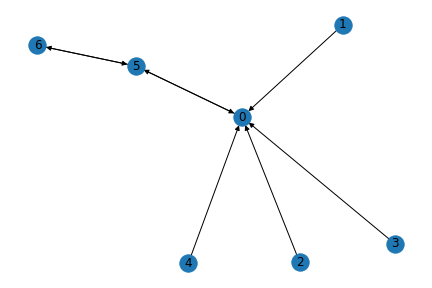
\includegraphics[width=0.55\linewidth]{figures/directed_graph_example_unranked.png}
  \caption{a weakly connected graph.}
  \label{fig:weaklyconnected}
\end{framed}
\end{figure}

In figure \ref{fig:weaklyconnectedpagedranked} we have the same
graph with vertex size and color indicating its PageRank with
parameter $\alpha=0.15$. We see that $5$ is ranked first, followed
by $0$. The smaller the restart parameter, the more important $5$
will get because we allow for longer paths with fewer restarts.

\begin{figure}[!htb]
\begin{framed}
  \centering
    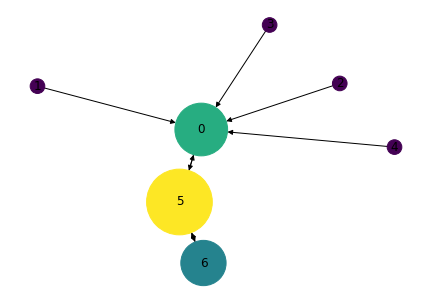
\includegraphics[width=0.55\linewidth]{figures/directed_graph_example.png}
  \caption{Pageranked graph.}
  \label{fig:weaklyconnectedpagedranked}
\end{framed}
\end{figure}

If we pick a restart parameter that is too large, which is the case
shown in figure \ref{fig:weaklyconnectedpagedrankedbadly}, the ranks
becomes almost uniform because the convex combination of the
original graph with the $n$-clique graph of the restarts is weighted
too heavily towards the latter. It also shows that for high restart
values $0$ becomes hotter than $5$. That is because paths of length
$\gt 2$ (before restart) become very unlikely in this random walk.

\begin{figure}[!htb]
\begin{framed}
  \centering
    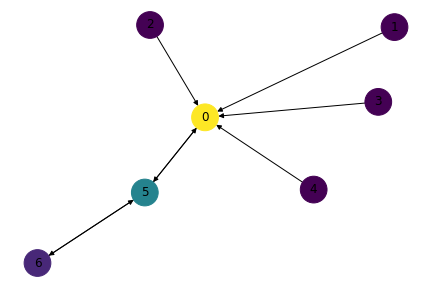
\includegraphics[width=0.55\linewidth]{figures/directed_graph_example_tinyalpha.png}
  \caption{again the same graph, with node color and size indicating
  their PageRank, with a restart probability approaching $1$.}
  \label{fig:weaklyconnectedpagedrankedbadly}
\end{framed}
\end{figure}

When we treat the same graph as undirected (figure
\ref{fig:undirectedanked} and calculate the PageRanks
($\alpha=0.15$), Vertex $0$ comes this time on top. It is more
central than $5$ and more random paths intersect it than any other
vertex.

\begin{figure}[!htb]
\begin{framed}
  \centering
    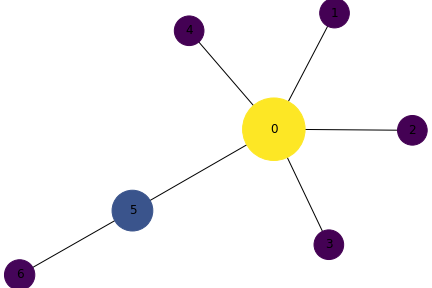
\includegraphics[width=0.55\linewidth]{figures/undirected_graph_example.png}
  \caption{same graph, but undirected.}
  \label{fig:undirectedanked}
\end{framed}
\end{figure}

In undirected graph, starts have hot centers and cold periphery.
a star has a hot center because it spreads its heat on many sources,
while each of the orbiting vertices sends all its heat into the star center.
The result is that hear accumulates at the center.

\begin{figure}[!htb]
\begin{framed}
\centering
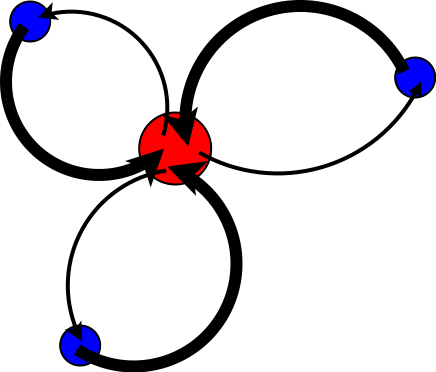
\includegraphics[width=0.55\linewidth]{figures/diagram_star.png}
\caption{a star graph.
}
\label{fig:hotstar}
\end{framed}
\end{figure}


